Given pattern `((number ...) ...)` and term `((1 2 3)())`, the matching algorithm should return `Match` instance with `number = ((1 2 3)())`, i.e. the pattern matches the term exactly. The diagram below shows how using `increasedepth` and `decreasedepth` methods provided by `Match` facilitate the matching. 

\begin{figure}[H]
\begin{subfigure}{0.5\linewidth}
	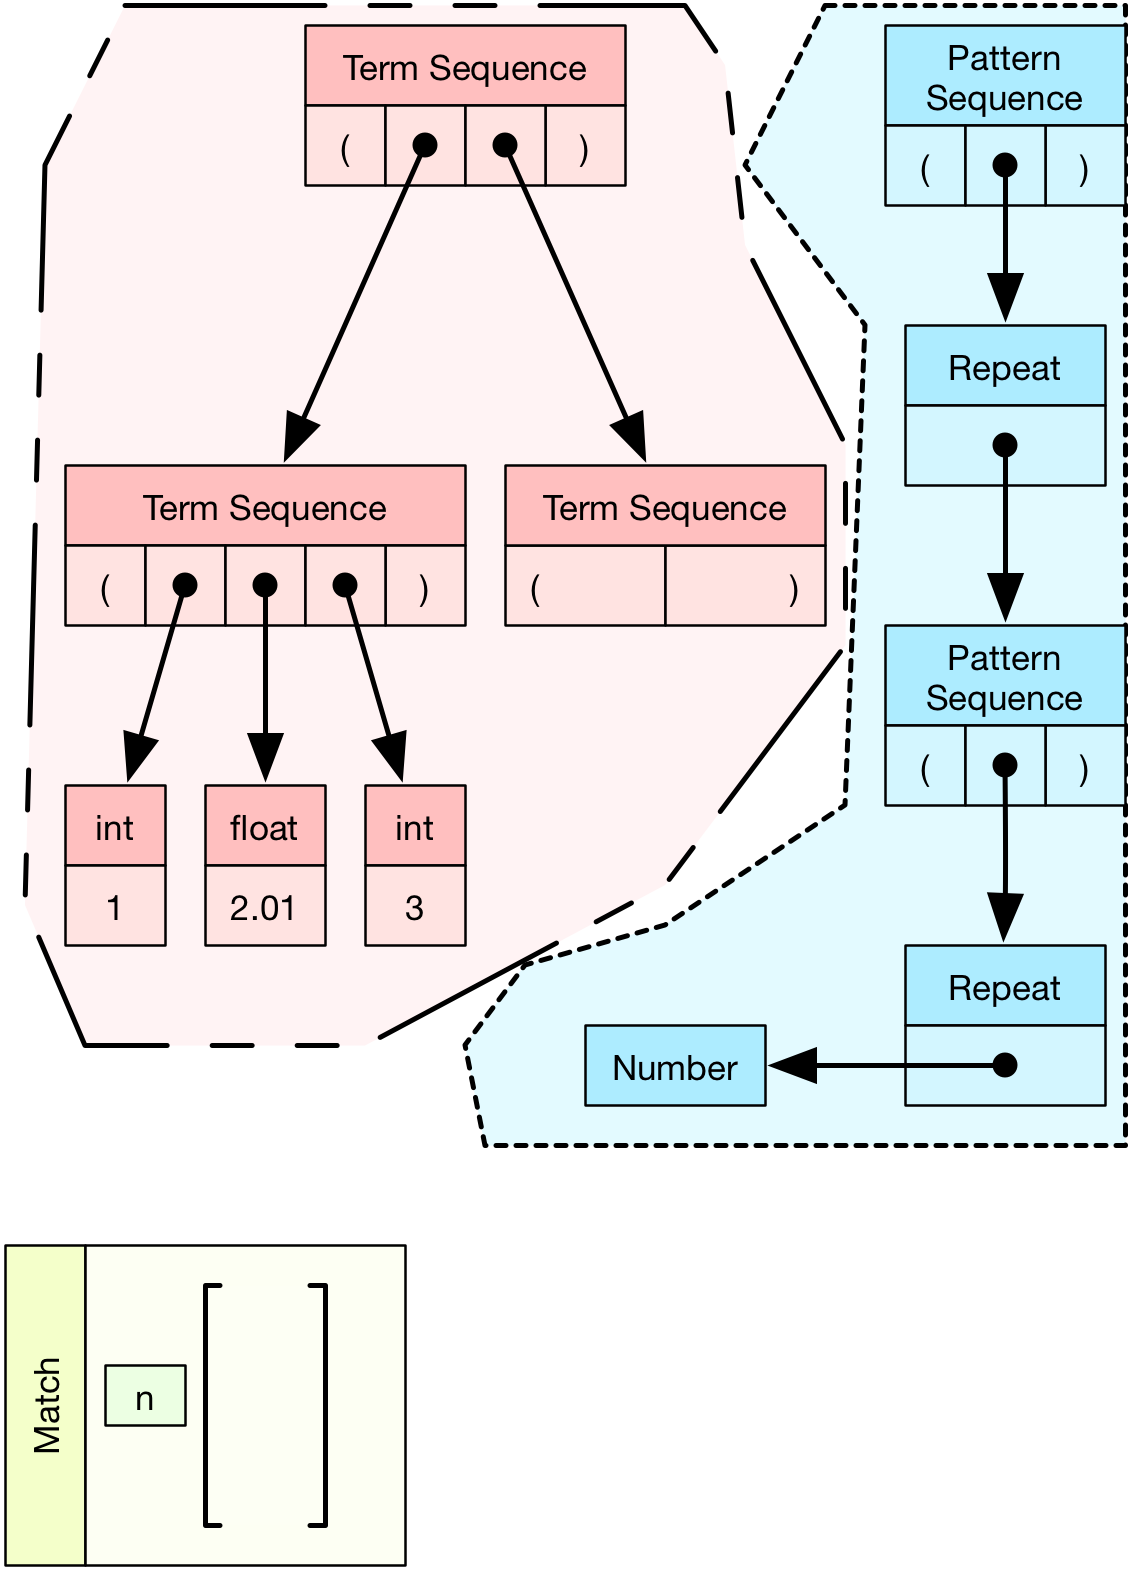
\includegraphics[scale=0.11]{ellipsis-example-fig-a.png}
	\caption{Before matching the pattern.}
	\label{ellipsis-example-fig-a}
\end{subfigure}
\begin{subfigure}{0.5\linewidth}
	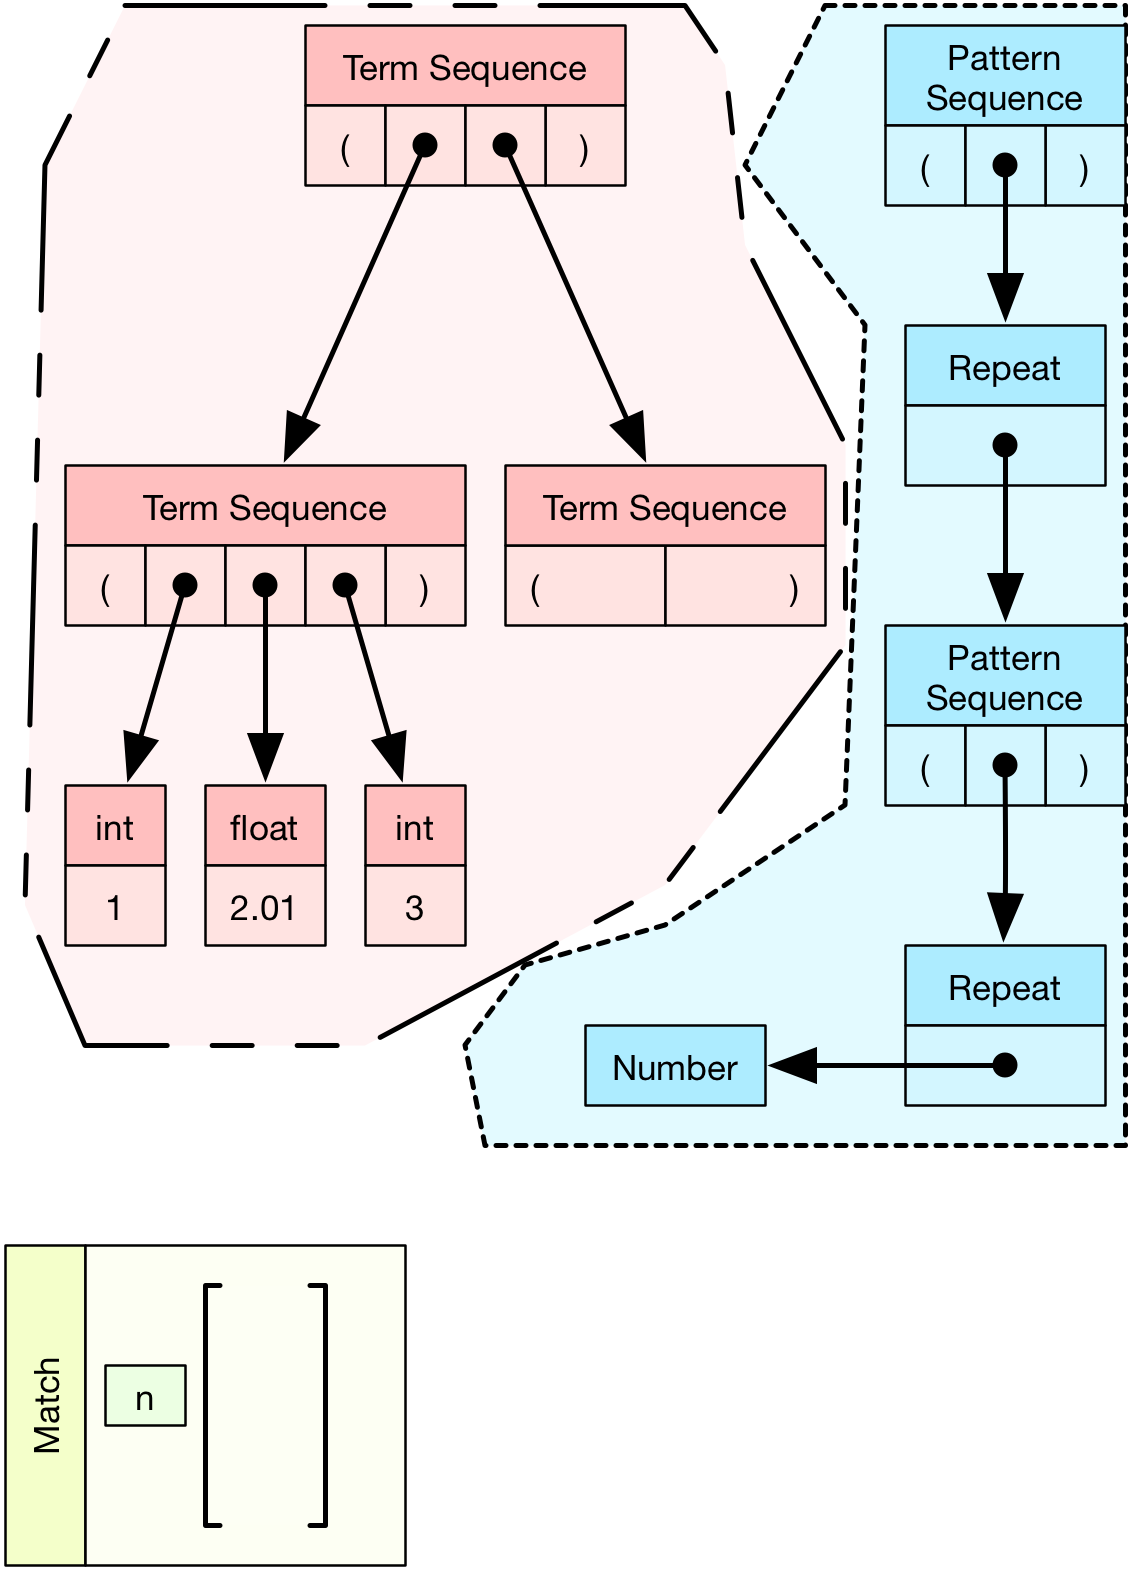
\includegraphics[scale=0.11]{ellipsis-example-fig-a.png}
	\caption{Before matching the pattern.}
	\label{ellipsis-example-fig-a}
\end{subfigure}

\caption{Hello}
\end{figure}
In Figure \ref{ellipsis-example-fig-a} one can see the state of the Match object before pattern matching. On the left the pattern and the term can be seen. Shadowed areas identify (terms being matches) TODO.  Stack of match object is empty.

Figure (b) shows state of the Match object after calling \texttt{increasedepth("n")} when matching \texttt{(n ...) ...}. New \texttt{TermSequence} instance is pushed onto the stack.

Figure (c) shows state of the Match object after calling \texttt{increasedepth("n")} when matching \texttt{n ...}. New \texttt{TermSequence} instance is pushed onto the stack.

Inner ellipsis now begins matching individual \texttt{n} terms. Figure (d) shows the state of the match after calling \texttt{addtobinding("n", Integer(1))}. Since topmost term on the stack is \texttt{TermSequence}, \texttt{Integer(1)} is appended.

Figures (e) and (f) show match object after matching 2.01 and 3, respectively.

Figure (g) shows match object after finishing to match inner ellipsis and calling \texttt{decreasedepth}. Since term before the topmost term is TermSequence, topmost TermSequence is appended to it. The remaining () now needs to be matched against pattern (n ...).

Figure (h) shows state of Match after starting to match inner ellipsis and calling increasedepth. This pushes empty sequence onto the stack.

Figure (i) shows state of Match after calling decreasedepth. This appends topmost sequence to the one below it.

Finally, there are no more terms to be matched by outer ellipsis, and decreasedepth depth is called. Since there's only one term on the stack, no action is performed.

This completes matching of a term. 

Of course, in ellipsis matching algorithm one may notice this example does not demonstrate all possible matches, but only lifetime of the only surviving match. In fact, after matching (1 2.01 3) against ( n ...) the following matches would be produced by ellipsis:

n =         0 3
n = ((1))   1 3
n = ((1 2)) 2 3
n = ((1 2 3)) 3 3
But the only one surviving is the one that has match all the terms. 

TODO 
